\documentclass[tikz,border=3mm]{standalone}
\usetikzlibrary{calc, arrows.meta}
\usepgfmodule{nonlineartransformations}

% Define the transformation to be employed
\makeatletter
\def\transformA{%
  \pgfmathsetmacro{\myX}{\pgf@x + 20*sin(-\pgf@y + .7*\pgf@x)}
  \pgfmathsetmacro{\myY}{\pgf@y + 20*cos(% .8\pgf@y +
    \pgf@x)}
  \setlength{\pgf@x}{\myX pt}
  \setlength{\pgf@y}{\myY pt}
}

% \def\transformB{%
  % \pgfmathsetmacro{\myRsq}{1/(sin(\pgf@x)*sin(\pgf@y) + 2)}
  % \pgfmathsetmacro{\myRsq}{1/(.001*\pgf@x*\pgf@x + .001*\pgf@y*\pgf@y + 1)}
  % \pgfmathsetmacro{\myX}{\pgf@x*e^(-\myRsq)}
  % \pgfmathsetmacro{\myY}{\pgf@y*e^(-\myRsq)}
  % \setlength{\pgf@x}{\myX pt}
  % \setlength{\pgf@y}{\myY pt}
% }

\makeatother

\begin{document}
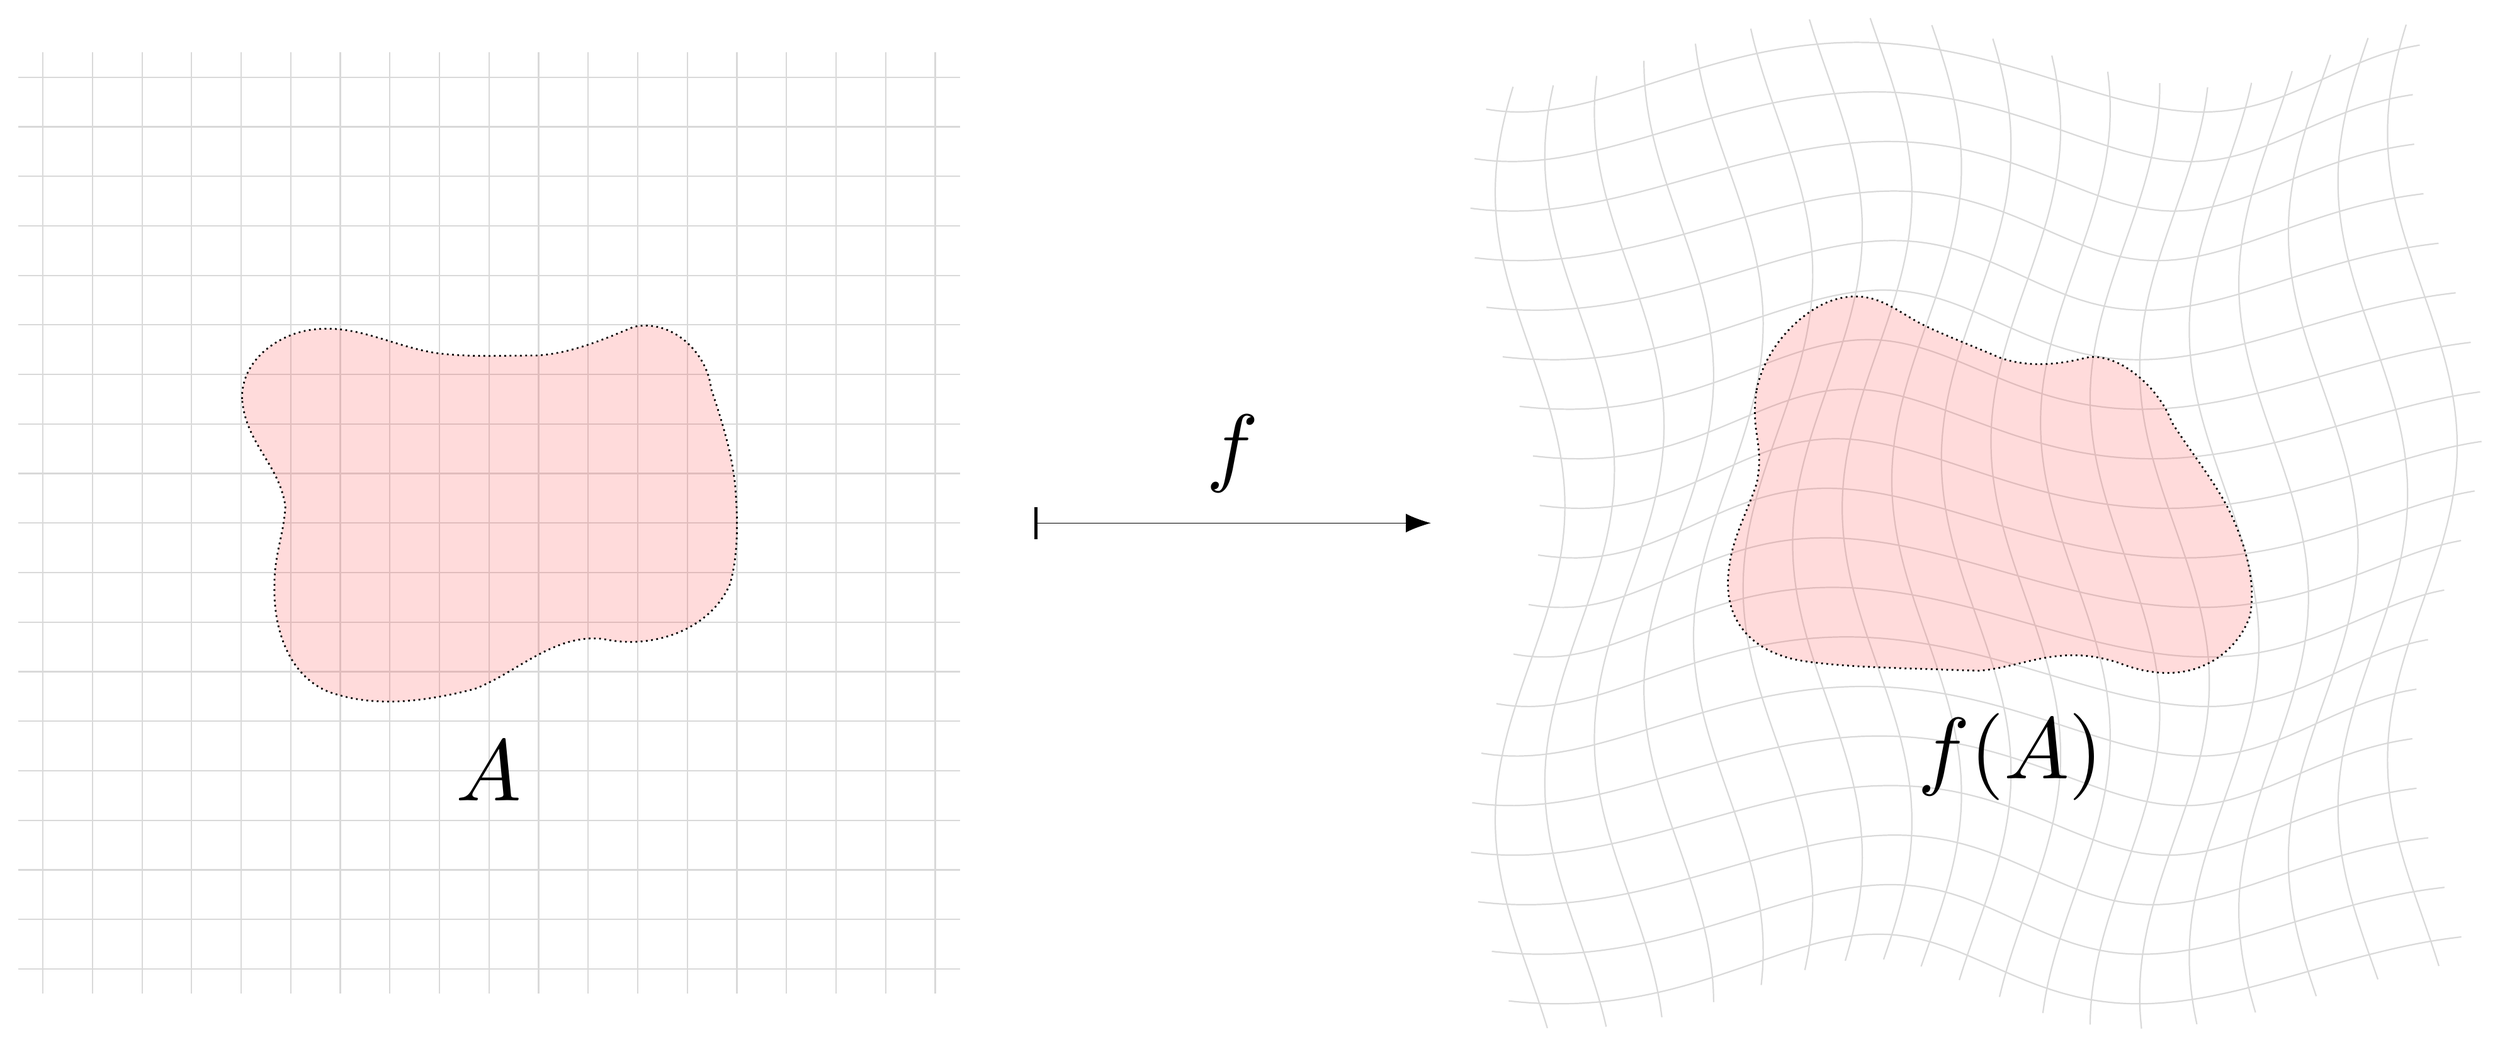
\begin{tikzpicture}[every node/.style={scale=5}]

  % Define xmin xmax ymin ymax
  \pgfmathsetmacro{\xmin}{-10}
  \pgfmathsetmacro{\xmax}{10}

  \pgfmathsetmacro{\ymin}{-10}
  \pgfmathsetmacro{\ymax}{10}

  \def\drawblob{
    \filldraw[draw=black, draw opacity=1, fill=red!70!white, fill opacity=.2, line
    width=1pt, dotted] (1.0090543497750044, -3.7475064639646534) -- (1.0090543497750044, -3.7475064639646534) .. controls (0.9967857429441586, -3.3371053391714534) and (1.414583424785918, -3.0572636303171494) .. (1.7903309096852034, -3.0410323056814423) -- (1.7903309096852034, -3.0410323056814423) .. controls (2.217158689036428, -3.0097485468797576) and (2.601518799729143, -3.2455252010474425) .. (3.019349212530858, -3.2900853794929246) -- (3.019349212530858, -3.2900853794929246) .. controls (3.3348276099053167, -3.326783408583613) and (3.6539525497705765, -3.3077626574749517) .. (3.9706279468262364, -3.309144204738778) -- (3.9706279468262364, -3.309144204738778) .. controls (4.318034291807611, -3.2910225151890216) and (4.641540956957284, -3.1532351882327756) .. (4.956758658474734, -3.020514761055034) -- (4.956758658474734, -3.020514761055034) .. controls (5.338876778398156, -2.933046597752692) and (5.70019778074493, -3.2743274859564027) .. (5.739396864713185, -3.6431558122954) -- (5.739396864713185, -3.6431558122954) .. controls (5.856644730417832, -3.9936883958860485) and (5.969603976501284, -4.349134462878869) .. (5.990124656644872, -4.7211674157566526) -- (5.990124656644872, -4.7211674157566526) .. controls (6.007798415168839, -5.018225033636421) and (6.0104469673341825, -5.325643936044153) .. (5.931335949165204, -5.613747092767667) -- (5.931335949165204, -5.613747092767667) .. controls (5.724903096521586, -6.0903437845026875) and (5.1334066575092505, -6.2765675890163735) .. (4.653434805494911, -6.16990689305698) -- (4.653434805494911, -6.16990689305698) .. controls (4.157390868324532, -6.111467251826695) and (3.785627953865152, -6.508113374670115) .. (3.3539625834255538, -6.674402328831797) -- (3.3539625834255538, -6.674402328831797) .. controls (2.8778338836272637, -6.79540673608915) and (2.355743781149603, -6.8731483651221446) .. (1.882257682433028, -6.702903540101281) -- (1.882257682433028, -6.702903540101281) .. controls (1.4615552638742473, -6.531882834553604) and (1.3186168581017217, -6.029598898243253) .. (1.3365860911273435, -5.6128073974657084) -- (1.3365860911273435, -5.6128073974657084) .. controls (1.3301336127057808, -5.345604702405504) and (1.434420754154592, -5.092151890083358) .. (1.4457905873821921, -4.8283790668777655) -- (1.4457905873821921, -4.8283790668777655) .. controls (1.3806470824396573, -4.3978677587310395) and (1.0474933587826407, -4.205211984637757) .. (1.0090543497750037, -3.747506463964652) -- cycle;
}

  \def\mydraw{
    \draw[help lines, color=gray!30, thick] ($(\xmin, \ymin) + (.5,
    .5)$) grid ($(\xmax, \ymax) + (-.5, -.5)$);
    \begin{scope}[xshift=-7cm, yshift=10cm, scale=2]
      \drawblob
    \end{scope}
  }

  \begin{scope}[xshift=-15cm]
    \mydraw
    \node () at (0,-5) {$A$};
  \end{scope}
  \draw[{Bar[scale=4, line width=2]}-{Latex[scale=3]}] (-4, 0) -- (4,0) node[midway, above] {$f$};
  \begin{scope}[xshift=15cm]
    \pgftransformnonlinear{\transformA}
    \mydraw
    \node () at (0,-5) {$f(A)$};
  \end{scope}

\end{tikzpicture}


\end{document}
